\chapter{Conception de la solution}
\label{Conception de la solution}

Ce chapitre se concentre sur l'architecture de l'application. Il inclut également une exploration approfondie de la conception, illustrée par des diagrammes techniques de classe et de séquence, en se basant sur les spécifications établies dans le deuxième chapitre.
\newpage

\section{Architecture de l'application}
\subsection{Architecture globale}

L'architecture e-commerce, telle que présentée ici, est volontairement simplifiée pour se concentrer sur les composants essentiels sur lesquels nous avons travaillé. Elle s’appuie sur plusieurs composants clés pour gérer les interactions entre le client, le contenu du site, les commandes et les paiements.
\begin{center}
    \centering
    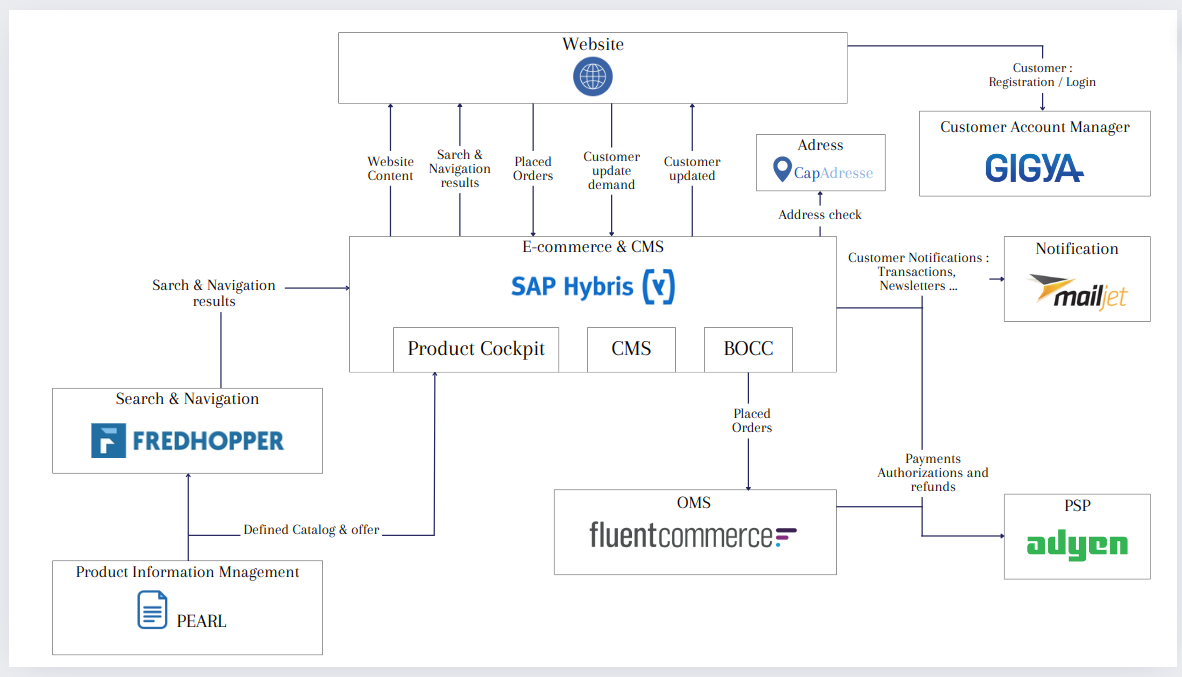
\includegraphics[width=19cm]{Figures/architectureGlobale.png}
    \captionof{figure}{Architecture globale de l'application E-commerce}
    \label{fig:processus}
\end{center}
\begin{itemize}
    \item [$\bullet$]Le site web permet aux clients de naviguer et de consulter le contenu (produits, offres, etc.). Le contenu est géré par le module CMS de SAP Hybris, qui centralise les informations et les affiches sur le storefront.
    \item [$\bullet$]Le moteur de recherche Fredhopper se charge de fournir les résultats de recherche et de navigation aux utilisateurs, en se basant sur les catalogues et les offres définis via PEARL, un système de gestion de l'information produit (PIM).
    \item [$\bullet$]Une fois la commande placée par le client via le site web, elle est prise en charge par SAP Hybris. Elle est ensuite transmise à Fluent Commerce, un système de gestion des commandes (OMS), qui suit et gère les différents statuts de la commande, depuis sa validation jusqu’à son expédition.
    \item [$\bullet$]CapAdresse est utilisé pour valider l’adresse du client avant la confirmation de la commande, afin de garantir la précision de la livraison.
    \item [$\bullet$]Mailjet est utilisé pour envoyer des notifications aux clients concernant les transactions, les newsletters, et d'autres communications, comme la confirmation de commande, d’expédition, ou d’annulation en cas de problème de paiement.
    \item [$\bullet$]Gigya s’occupe de la gestion des comptes clients, notamment l’enregistrement et la connexion des utilisateurs sur le site.
\end{itemize}
Lorsqu'un client effectue un paiement sur le site, une requête est envoyée à Adyen pour obtenir une autorisation. Adyen traite la demande et renvoie une réponse indiquant si le paiement est "autorisé" ou "non autorisé". Si le paiement est refusé, le client est redirigé vers une page d'erreur. En revanche, si le paiement est approuvé, le client est dirigé vers la page de confirmation de commande, et simultanément, la commande est exportée vers Fluent Commerce, le système de gestion des commandes.Fluent Commerce est chargé de gérer le cycle de vie de la commande en attendant la notification d'Adyen confirmant que le paiement a bien été autorisé, car il peut être annulé en cas de fraude ou de problème de sécurité. Si la notification indique que le paiement a été annulé, Fluent communique avec Mailjet pour envoyer un e-mail d'annulation au client. Cependant, si le paiement est confirmé, un e-mail de confirmation de commande est envoyé via Mailjet. Par la suite, une fois la commande prête à être expédiée, Fluent envoie une requête de capture à Adyen. Dès qu'Adyen confirme que la capture a été effectuée avec succès, la commande est expédiée, et Mailjet envoie un e-mail de confirmation de livraison au client. En plus de ces tâches, Fluent Commerce prend également en charge plusieurs aspects logistiques de la commande, tels que la vérification de la disponibilité des produits, la gestion des entrepôts pour l’expédition, ainsi que le suivi du statut de la commande (en attente, en préparation, expédiée, etc.).

\subsection{Architecture backend simplifiée}
Notre solution est basée sur la plate-forme SAP Hybris Et suit donc l'architecture presentée ci-dessous :
\begin{center}
    \centering
    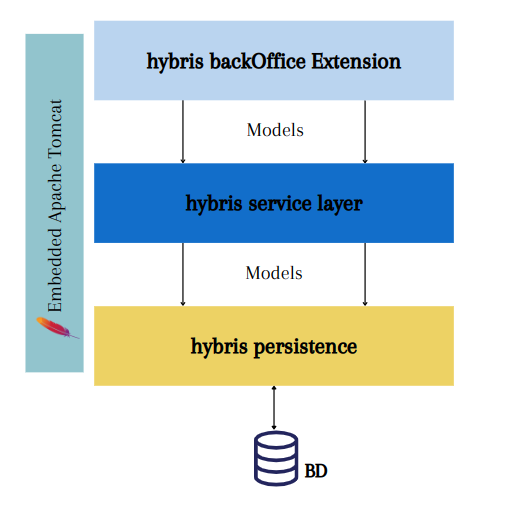
\includegraphics[width=14cm]{Figures/architecturebacend.png}
    \captionof{figure}{Architecture backend simplifiée de l'application E-commerce}
    \label{fig:processus}
\end{center}

\begin{itemize}
    \item [$\bullet$]\textbf{Serveur Apache Tomcat:} La plateforme Hybris utilise Apache Tomcat comme serveur HTTP intégré. Ce serveur d'application est responsable de l'hébergement de l'application Hybris et de la gestion des requêtes HTTP/HTTPS entrantes, assurant ainsi le bon fonctionnement de l'application web.
    \item [$\bullet$]\textbf{Extension Backoffice de Hybris:} L'extension Backoffice est une composante essentielle de Hybris qui permet aux utilisateurs métiers d'accéder aux fonctionnalités d'administration de contenu. Cela inclut la gestion du catalogue, des catégories, des produits, ainsi que des entités et types du système. Cette extension fournit une interface graphique conviviale pour les utilisateurs finaux, facilitant la gestion et l'organisation des données. En outre, elle offre aux développeurs la possibilité de créer ou de personnaliser des composants Hybris en fonction des besoins spécifiques de l'entreprise.
    \item [$\bullet$]\textbf{Service Layer de Hybris: }La couche de service (Service Layer) représente la couche métier de l'application Hybris, où est implémentée la logique de gestion d'entreprise. Elle est constituée d'un ensemble de services qui encapsulent les règles métiers et les processus de l'entreprise. La couche de service communique à la fois avec l'extension Backoffice et la couche de persistance via des modèles, qui sont des représentations des entités de la logique métier. Ces modèles servent d'intermédiaires entre les différentes couches, facilitant ainsi la manipulation des données de manière cohérente et sécurisée.
    \item [$\bullet$]\textbf{Couche de Persistance de Hybris:} La couche de persistance est le composant qui assure l'interaction entre le Service Layer et la base de données. Elle est responsable de la gestion de toutes les opérations de lecture et d'écriture dans la base de données, garantissant que les données sont stockées de manière efficace et peuvent être récupérées de manière fiable. 
\end{itemize}

\subsection{Environnent de livraison et de test }


Cette section présente le processus de déploiement du projet, en détaillant les différents serveurs utilisés. La structure se compose de deux parties principales : interne et externe.

\begin{center}
    \centering
    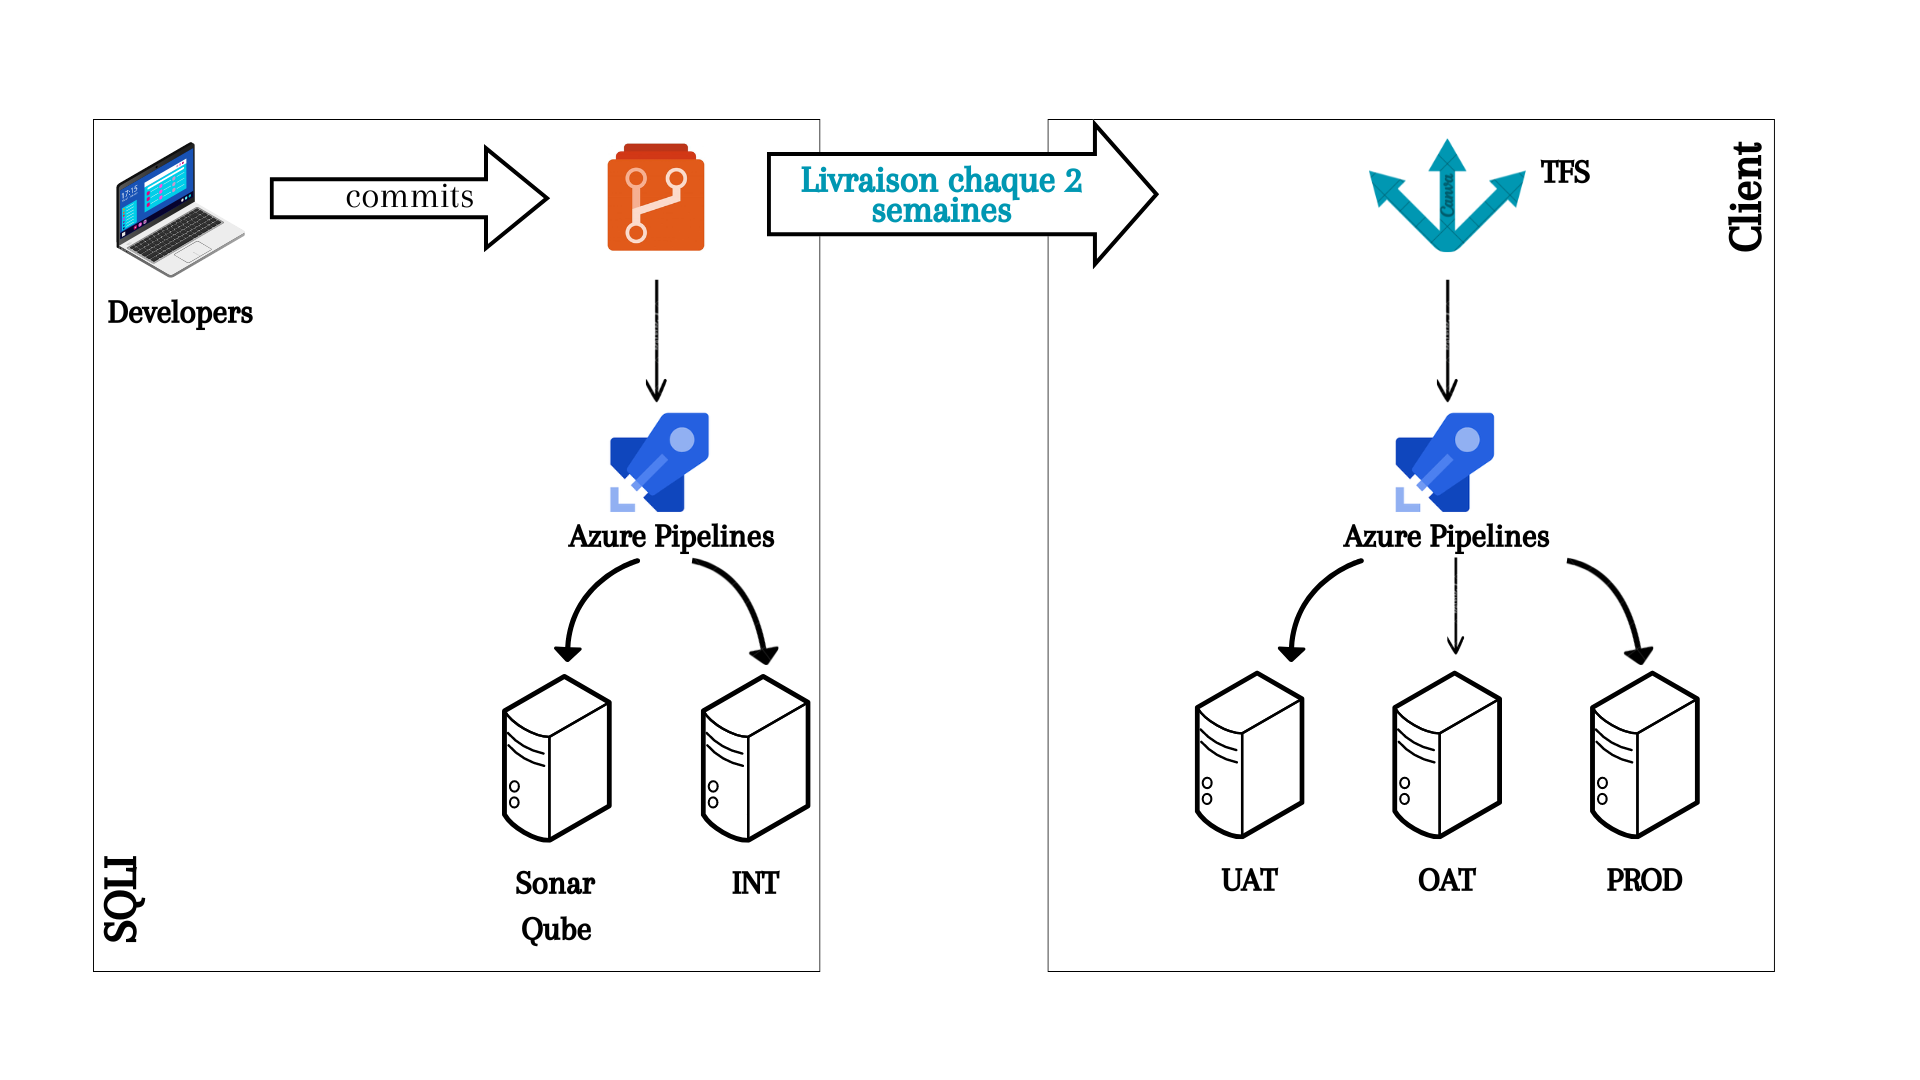
\includegraphics[width=19cm]{Figures/Test.png}
    \captionof{figure}{Architecture de livraison et de test simplifiée}
    \label{fig:processus}
\end{center}
\begin{center}
    \centering
    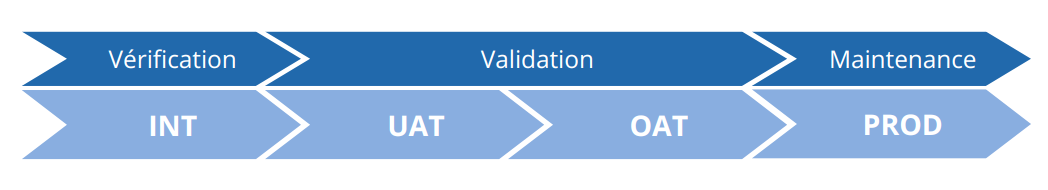
\includegraphics[width=19cm]{Figures/UAT.png}
    \captionof{figure}{Environnements de test et production}
    \label{fig:processus}
\end{center}



\subsubsection{Architecture interne}
L'architecture interne est implémentée au sein de SQLI et comprend un serveur d'intégration (INT) et un serveur SonarQube pour l'analyse de la qualité du code. Les développeurs effectuent des commits sur le dépôt Azure DevOps, puis un serveur d'intégration continue, Jenkins, récupère les dernières versions depuis ce dépôt pour effectuer une compilation automatique avec ANT. Jenkins lance ensuite une analyse SonarQube pour garantir la qualité du code. Après l'analyse SonarQube, le serveur vérifie que le nombre d'erreurs détectées ne dépasse pas les limites prédéfinies en fonction de la gravité des erreurs et des quotas définis sur le serveur SonarQube. Si ces contrôles sont satisfaits, Jenkins déploie le code sur le serveur d'intégration (INT). Ce processus d'intégration continue se répète tout au long du sprint de trois semaines.


\subsubsection{Architecture externe}

L'architecture externe est implémentée dans l'environnement du client et se compose de trois serveurs : UAT (User Acceptance Testing), OAT (Operational Acceptance Testing) et PROD (Production). Toutes les deux semaines, une nouvelle version est livrée dans le système de gestion de versions du client, TFS (Team Foundation Server).

\begin{itemize} \item [$\bullet$]\textbf{Serveur UAT:} Utilisé pour tester les livrables et s'assurer qu'ils répondent aux attentes de l'utilisateur final. \item [$\bullet$]\textbf{Serveur OAT:} Permet de déterminer si les livrables sont opérationnels et prêts à être intégrés dans l'environnement de production. \item [$\bullet$]\textbf{Serveur PROD:} Après les processus de test, une mise en production (MEP) est effectuée tous les trois mois, rendant la version finale disponible pour les utilisateurs finaux. \end{itemize}

\subsection{Architecture applicative}

Dans le cadre de l'utilisation de la solution Hybris, il est conseillé de suivre l'architecture applicative qu'elle propose. Cette architecture est basée sur un modèle n-tiers largement utilisé dans les applications web, permettant une répartition claire des rôles et une meilleure structuration du code. Quatre principaux patrons de conception sont au cœur de cette architecture :

\begin{center}
    \centering
    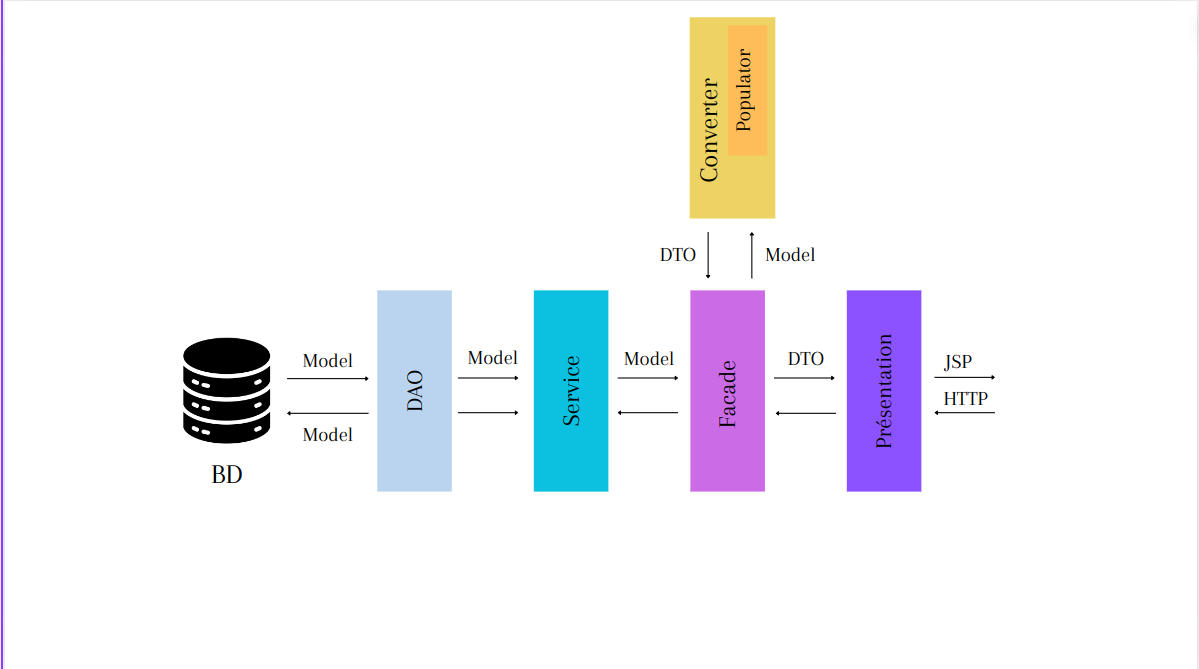
\includegraphics[width=19cm]{Figures/Dto.png}
    \captionof{figure}{Architecture applicative de l'application E-commerce}
    \label{fig:processus}
\end{center} 

\begin{itemize}
    \item[$\bullet$] \textbf{Modèle MVC (Modèle-Vue-Contrôleur)} : Ce modèle permet de séparer distinctement la présentation, la logique métier et l'accès aux données. Cela garantit une organisation modulaire, rendant l'application plus facile à maintenir et à étendre. Par exemple, dans notre application, la vue pourrait être gérée par des pages JSP ou des composants front-end, tandis que les contrôleurs orchestrent les opérations de la logique métier encapsulée dans les services.

    \item[$\bullet$] \textbf{Patron de Façade} : Ce patron simplifie l'accès à un système complexe en fournissant une interface unique qui masque la complexité des sous-systèmes sous-jacents. Dans notre projet, la façade centralise les interactions entre la couche de services et la couche de présentation. Elle reçoit des objets modèles depuis les services, les transforme en DTO grâce à des Converters et Populators, et les transmet à la couche de présentation. Cette approche améliore la modularité et facilite la gestion des données au sein du système.

    \item[$\bullet$] \textbf{Patron DAO (Data Access Object)} : Ce patron permet d'accéder aux données sans être lié à un SGBD spécifique, en fournissant une abstraction qui rend l'application plus flexible. Il encapsule la logique d'accès aux données, permettant d'intégrer facilement différents SGBD sans modifier le code de l'application. Par exemple, le DAO pour "Produit" ou "Client" peut contenir toute la logique nécessaire pour interagir avec les données associées, indépendamment de la base utilisée.

    \item[$\bullet$] \textbf{Patron DTO (Data Transfer Object)} : Ce modèle optimise les échanges de données entre différentes couches de l'application en regroupant les informations dans des objets spécifiques. Il permet de réduire la surcharge de transfert de données, améliorant ainsi l'efficacité des communications entre les couches. Dans notre application, les DTO servent de pont entre la couche de service et la présentation, réduisant les dépendances et simplifiant les tests unitaires.
\end{itemize}

Adopter cette architecture permet non seulement une meilleure organisation du code, mais aussi d'assurer une évolutivité et une maintenance aisée à long terme.
\section{Conception detaillée}

\subsection{Diagramme de classe}
\begin{center}
    \centering
    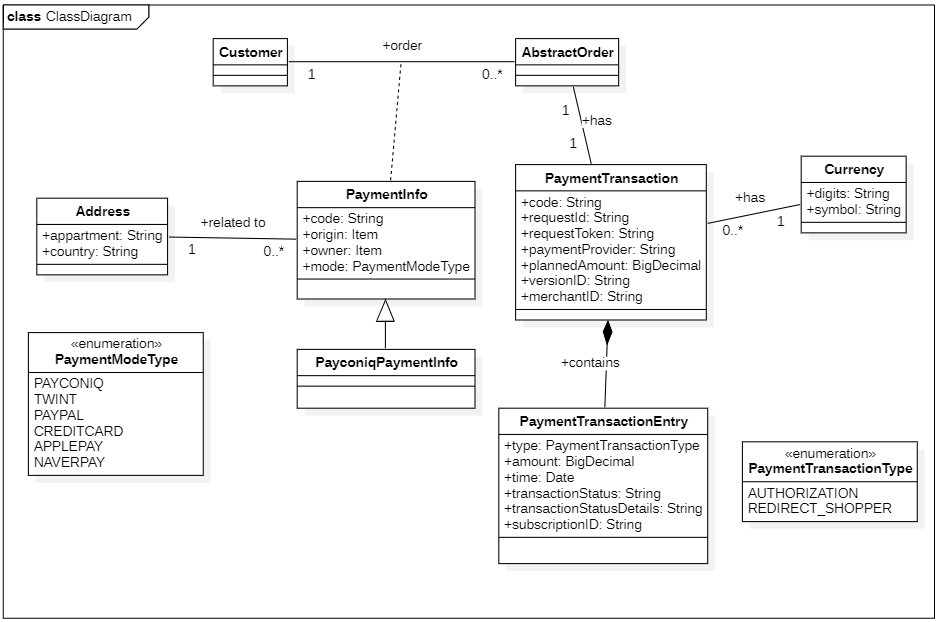
\includegraphics[width=19cm]{Figures/class.png}
    \captionof{figure}{Diagramme de classe}
\end{center}

La figure ci-dessus représente le diagramme de classe de notre système. Un Client peut passer plusieurs Commandes (représentées par la classe AbstractOrder), et chaque commande est associée à une Transaction de paiement (PaymentTransaction). Cette transaction contient des détails tels que le fournisseur de paiement, le montant prévu, et les identifiants du marchand. Elle est liée à une ou plusieurs Entrées de transaction (PaymentTransactionEntry), qui décrivent des aspects spécifiques comme le type de transaction, le montant, l'heure, et l'état de la transaction. Les informations de paiement sont représentées par la classe PaymentInfo, qui inclut le mode de paiement (défini par l'énumération PaymentModeType), et peut être associée à une Adresse. Une spécialisation de PaymentInfo, nommée PayconiqPaymentInfo, est utilisée pour les transactions via Payconiq. Le système gère également les devises via la classe Currency, qui est associée aux transactions de paiement. En somme, ce diagramme modélise la partie structurelle d'un volet de la gestion de paiement dans notre site e-commerce où les clients effectuent des paiements par divers moyens.

\subsection{Diagramme de séquence}

\begin{center}
    \centering
    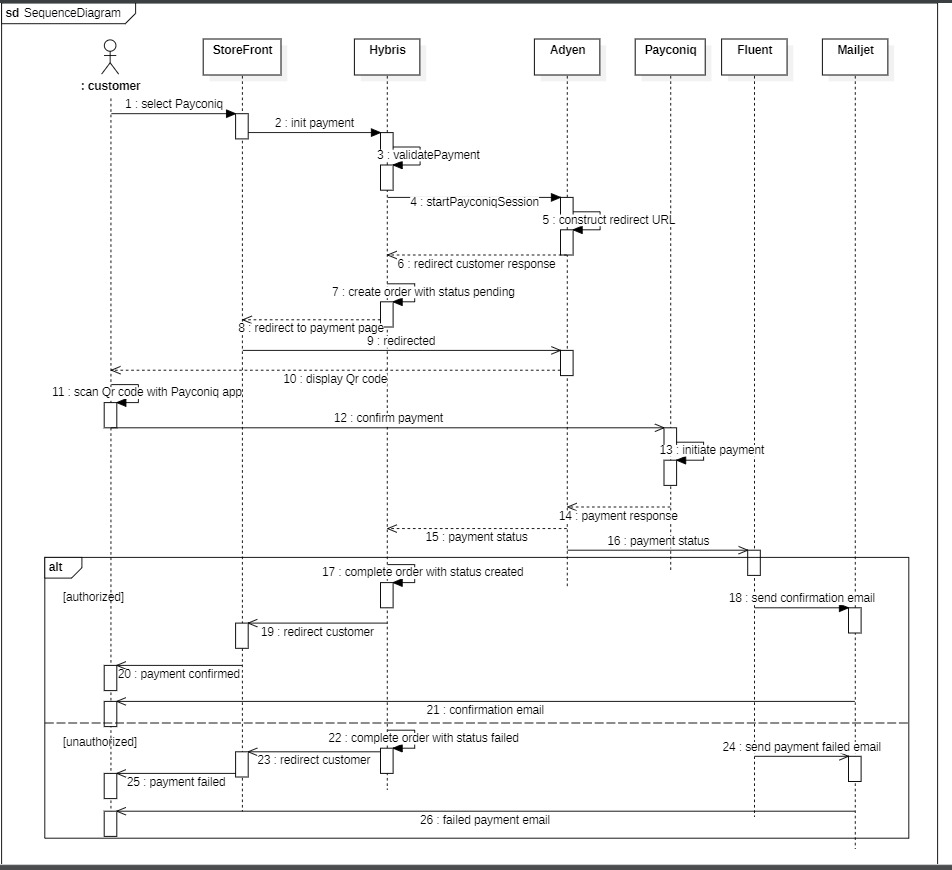
\includegraphics[width=19cm]{Figures/sequence.png}
    \captionof{figure}{Diagramme de séquence }
    \label{fig:processus}
\end{center} 


Le processus de paiement via Payconiq commence lorsque le client sélectionne ce moyen de paiement sur la plateforme. La transaction est alors initialisée et validée pour s'assurer que toutes les conditions sont remplies. Ensuite, une session Payconiq est démarrée via Adyen, qui génère une URL de redirection pour amener le client à la page de paiement Payconiq. Une fois redirigé, une commande est créée avec le statut "en attente". La page de paiement affiche un QR code que le client doit scanner avec son application Payconiq. Après avoir scanné le QR code, la confirmation du paiement est envoyée de Payconiq à Adyen, qui informe ensuite la plateforme e-commerce du statut du paiement.

Si le paiement est autorisé, la commande est complétée avec le statut "créée", le client est redirigé vers une page de confirmation, et un e-mail de confirmation de commande est envoyé. En revanche, si le paiement échoue, la commande est marquée avec le statut "échec", le client est redirigé vers une page d'échec de paiement, et un e-mail d'échec de paiement est envoyé.



\subsection*{Conclusion}

Ce chapitre a été dédié à l’étude conceptuelle du projet. Après une présentation des architectures adoptées et des diagrammes techniques de classe et de séquence, une compréhension approfondie du projet a été acquise. La prochaine étape consistera à aborder l’implémentation et la validation de la solution, sujet du chapitre suivant.
\pagebreak